\chapter{Feature-based approach}
\label{cha:FeatureApproach}

%TODO: why features? adding another important information to point coordinates --> curvature of points

To solve the main drawbacks of finding reliable point correspondences between $C_1$ and $C_2$ the focus lies on point features for an initial alignment as they provide meaningful information about a point $p$ being compared to its neighbors. The approach to use point features for the non-rigid registration procedure is closely related to Mitra \cite{Mitra07}. The main part thereby is the computation of point feature histograms, namely ``Fast point feature histograms'' (FPFH) \cite{FPFH}. Basically, the computed features describe the curvature between specific points. By computing those features for all points, depending on the curvature, which might be an implied curve for an ellipsoid rigid part, in case of intersections of rigid parts, different features are proposed. Taking only \textit{unique} feature histograms for correspondence estimation which are features considerably deviating from the mean histogram $\mu$ of all point feature histograms of a cluster $C_i$  allows to reduce computation time. It is thereby assumed that those unique features are those located between rigid parts.

\section{Fast point feature histograms}
\label{FPFH}
The ``Fast Point Feature histograms'' (FPFH) algorithm is an improved approach of the `'Persistent Point Feature Histogram for 3D Point Clouds'' \cite{PPFH}. It focuses on computing features, depending on a points normal $\vec{n}$ and its $k$ neighbors.  The choice of those features are the following: 
%%
\begin{itemize}
	\item rotation- and scale-invariant features
	\item easy comparison of feature histograms
	\item straightforward implementation
	\item approval of approach
	\item easy adaption from different dimensions (2D and 3D)
\end{itemize}
%%
By using a histogram the neighborhoods' geometrical properties can be provided in form of the mean surface curvature at a point $\boldsymbol{p}$. As in the unordered list of points no surface and following no point normals are provided, those have to be computed in a initial step (see subsection \ref{normal}).

\subsection{Normal estimation}
\label{normal}

As a first step, the normals of all unordered points from the input clusters $C_1$ and $C_2$ need to be estimated \cite{normals}. Those is achieved by taking all points $k$ within a radius $r$ from a point $\boldsymbol{p}$. Subsequently, a least error fit straight line $X$ in the form $ax + by +c = 0$ to all $k$ points is computed by minimizing the squared distances from all points $\boldsymbol{p_i(x_i,y_i)}$
%%
\begin{equation}
\begin{split}
dist^2(x_i, y_i) = (ax_i + by_i + c)^2
\\
e =   \displaystyle\sum_{i=1}^{k} dist^2(x_i, y_i)
\end{split}
\end{equation}
%%
to $X$. This is done by computing the unknown parameters $a, b$ of $X$ with the covariance matrix 
%%
\begin{equation}
\begin{pmatrix}
\overline{x^2} - \overline{x} \cdot \overline{x} & \overline{xy} -\overline{x} \cdot \overline{y}\\
\overline{xy} -\overline{y} \cdot \overline{x} & \overline{y^2} -\overline{y} \cdot \overline{y}
\end{pmatrix} \cdot \begin{pmatrix}
a \\
b
\end{pmatrix} = \lambda \cdot \begin{pmatrix}
a \\
b
\end{pmatrix}
\end{equation}
%%
resulting in two pairs of an eigenvalue and eigenvector $(n_1,\lambda_1)$ and $(n_2,\lambda_2)$. The normal of $\boldsymbol{p}$ is computed solving the linear equation for the normal vector $\vec{n_2}$ which is represented by $\lambda_2$. The procedure is conducted for all points from $C_1$ and $C_2$ (see figure \ref{fig:normalEstimation}). 
%%
\begin{figure}[H]
	\centering
	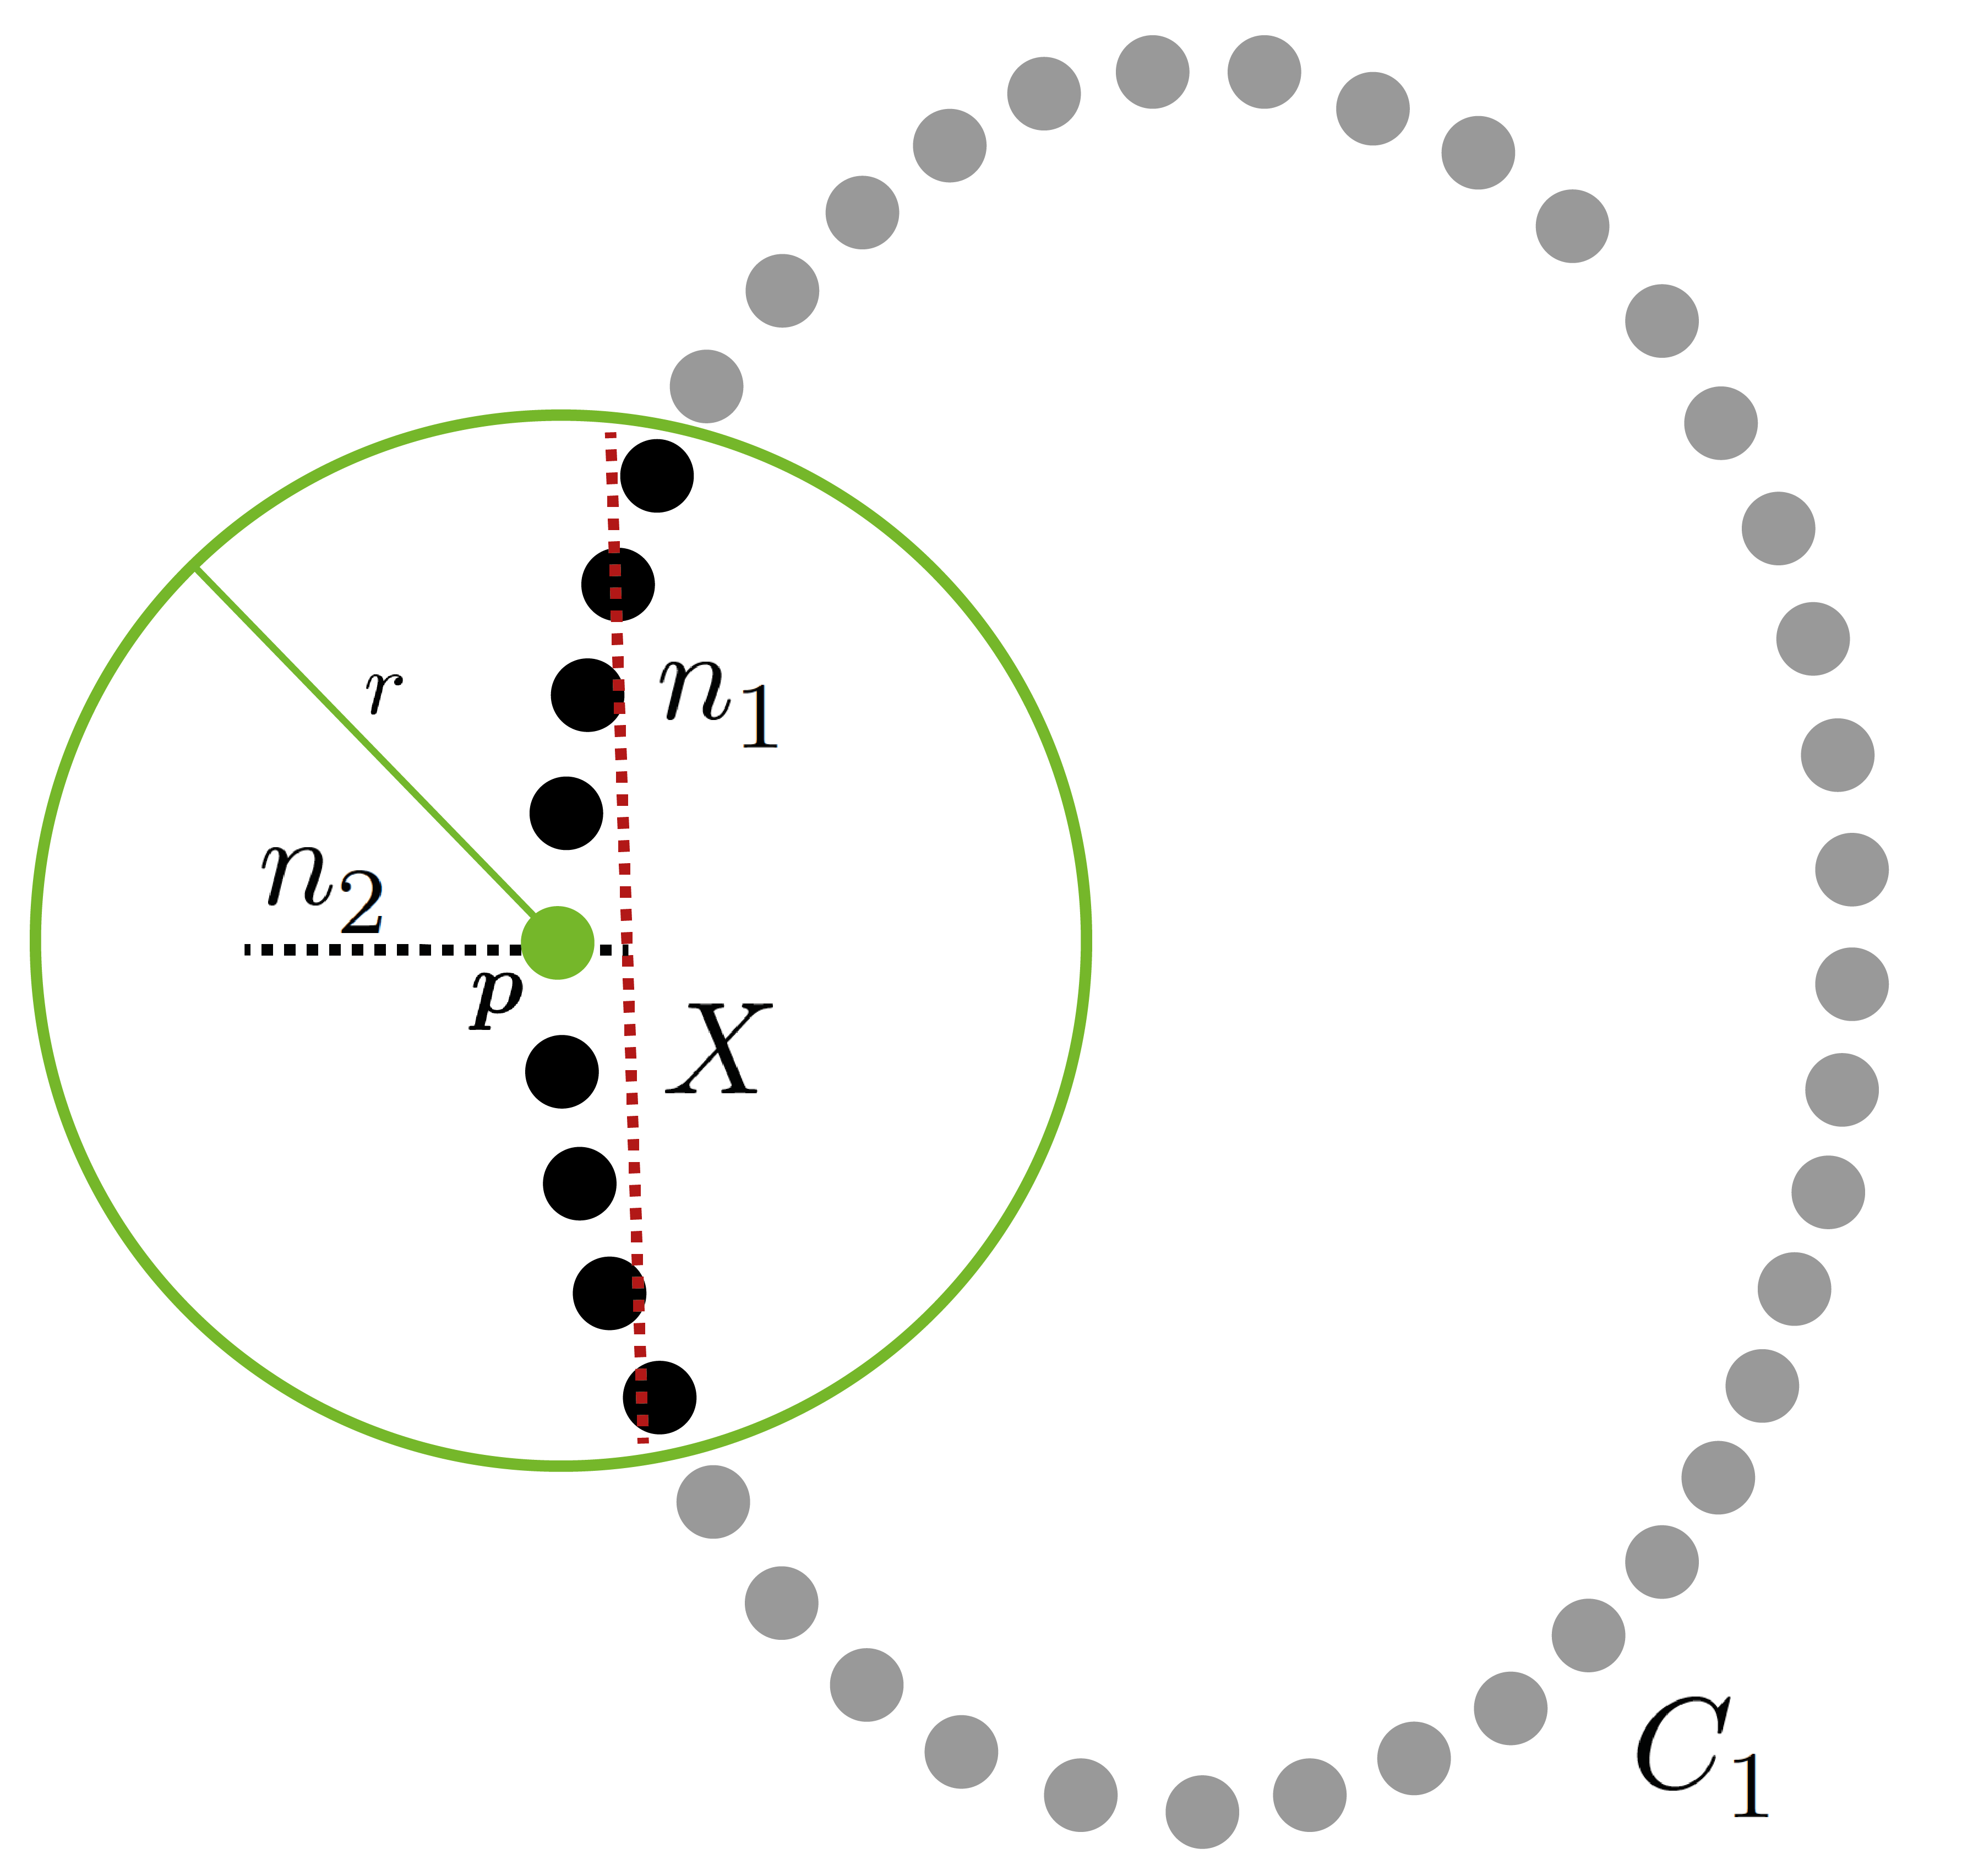
\includegraphics[width=0.4\linewidth]{normalEstimation}
	\caption{Normal estimation for a cluster point $\boldsymbol{p}$ of $C_i$ by a computation of the least squared fitting line $X$ of the neighborhood inside a radius $r$. Calculation of the eigenvectors $\vec{n_1}$ and $\vec{n_2}$ by the covariance matrix of all $k$ points.}
	\label{fig:normalEstimation}
\end{figure}
%%
As a next step, it is required that all normals are equally oriented. Basically, all $n$ computed normals are traversed globally, starting with a normal $\vec{n_i}$ of a point $p_i$. Thereby, it is of particular importance to select a normal that assures consistent orientations between $C_1$ and $C_2$. Taking its orientation as parent normal $\vec{n_p}$, the angle $\delta$ between $\vec{n_p}$ and all neighboring normals $\vec{n_k}$ 
%%
\begin{equation}
\delta = \vec{n_p} \cdot \vec{n_k}, \quad \text{for $|\vec{n_p}|, |\vec{n_k}| = 1$}
\end{equation}
%%
is computed. In case of $\delta < 0$, $\vec{n_k}$ requires to be flipped 180° ($\vec{n_k} = -\vec{n_k})$. If all $k$ normals have been verified to be oriented in consideration of $\vec{n_p}$ any $\vec{n_k}$ is selected as current $\vec{n_p}$. The whole algorithm proceeds until all $n$ normals have been verified to correspond with their parent normal $n_p$.

\subsection{SPFH and FPFH}
The simplified point feature histogram (SPFH) for a point $\boldsymbol{p}$ is then computed by using three geometric features. Between $\boldsymbol{p}$ and each of its $k$ neighbors $\boldsymbol{p_k}$ given a threshold $\tau$, those features are computed -- $\boldsymbol{p_i}$ is thereby the point having the smaller angle between its normal and the line connecting the point set, $\boldsymbol{p_j}$ corresponds to the remaining point. Using their normals $n_i$ and $n_j$ a Darboux $uvn$ frame $(u = n_i, v = (p_j - p_i) \times u, w = u \times v)$ is computed. The following angles
%%
\begin{equation}
\begin{split}
\alpha = v \cdot n_j
\\
\phi = (u \cdot (p_j - p_i))/\|p_j - p_j\|
\\
\theta = arctan(w \cdot n_j, u \cdot n_j)
\end{split}
\label{eq:AngularVariations}
\end{equation}
%%
are computed. In a second step for each point $\boldsymbol{p_i}$ again all $n$ neighbor points given a threshold $\tau$ are computed. The simple point histogram SPF of $p$ is then weighted to the final histogram
%%
\begin{equation}
FPFH(\boldsymbol{p}) = SPF(\boldsymbol{p}) + \frac{1}{n} \cdot \displaystyle\sum_{i=1}^{n}\frac{1}{w_i} \cdot SPF(p_i)
\end{equation}
%%
where the weight $w_i$ represents the distance $d(\boldsymbol{p},\boldsymbol{p}_i)$. The influence region diagram for a Fast Point feature histogram for a query point $\boldsymbol{p_q}$ can be seen on Figure \ref{fig:FPFHregion}. 
%%
\begin{figure}[H]
	\centering
	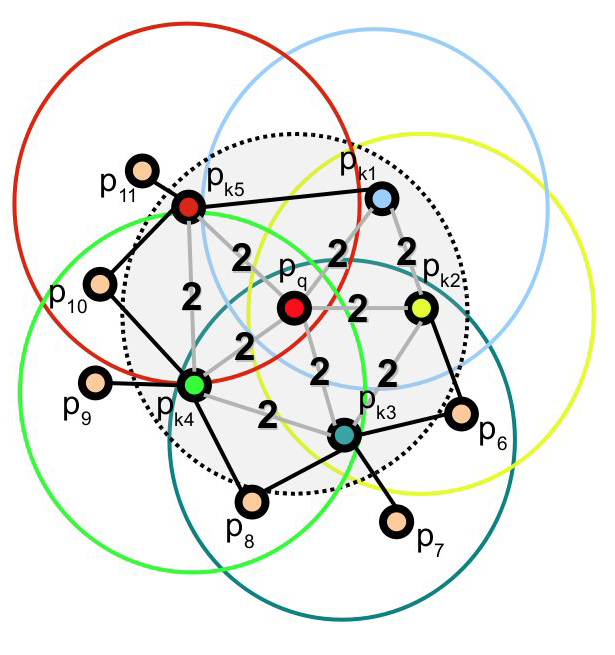
\includegraphics[width=0.4\linewidth]{FPFH_region}
	\caption{The point region for the calculation of the feature histogram for a query point $\boldsymbol{p}_q$. The histogram of $\boldsymbol{p}_q$ and its neighbors (inside the grey circle) is weighted with the further linked neighbors (colored circles) \cite{FPFH}.}
	\label{fig:FPFHregion}
\end{figure}
%%
\subsection{Creation of feature histograms}
The resulting feature values for each point $p$ of $C_1$ and $C_2$ in form of three angles between its neighbors $k$ are categorized using a histogram $H \{bin_1,\ldots,bin_b\}$ with $b = q^f$ bins to consider all possible combinations of the feature values. Thereby, $q$ represents the number of intervals and $f$ the number of feature values, in this case 3. After the allocation the associated bin at the index $idx$
%%
\begin{equation}
idx = \displaystyle\sum_{i=1}^{i \leq f}q(f_i) \cdot 2^{i-1}
\end{equation}
%%
is incremented by 1. The function $q(f)$ returns the interval the feature is allocated to, ranging from 0 to $q - 1$. Finally, each bin contains the number of point pairs that are allocated in the specified value interval.As soon as the feature histograms of all points from $C_1$ and $C_2$ are computed only salient histograms are taken as comparison for point correspondence between $C_1$ and $C_2$ to safe computation time. In order to achieve that the mean of all feature histograms $\mu$ of a cluster $C_i$ is computed. Subsequently, the distance of a feature histogram $H_i$ is compared to $H_\mu$ and in case of being outside the value $\mu \pm \sigma$ denoted as \textit{unique} and passed to the next step of detecting matching histograms between $C_1$ and $C_2$. The standard deviation
%%
\begin{equation}
\sigma = \frac{1}{N} \cdot \displaystyle\sum_{i=1}^{N}(H_i(b) - \overline{H_i})^2
\end{equation}
%%
is therefore calculated for all histograms $H_i$ with $N$ data entries of all cluster points. 
%%
\subsection{Comparison of histograms}
\label{histogramCriteria}

As a next step, all \textit{unique} feature histograms of $C_1$ are verified to find the closest match from $C_2$. For that reason, different histogram-similarity criteria have to be determined to measure the similarity between two histograms $H_j$ and $H_k$ with each $b$ bins. In order to detect the best fitting histogram three main criteria mentioned most often in reference papers \cite{surfletPairRelation} \cite{localFeatureHistograms} were selected. As first criterion the squared euclidean distance (L2)
%%
\begin{equation}
\varepsilon(H_j, H_k) = \displaystyle\sum_{i=1}^{b}(H_j(i) - H_k(i))^2
\end{equation}
%%
is computed. In the reference paper of Mitra et al. \cite{Mitra07} the euclidean distance was the only criterian for correspondence computation which generates most of the point correspondences (see section \ref{ResultsLRP}). Subsequently, the statistical Chi-Square ($\chi^2$) divergence
%%
\begin{equation}
\chi^2(H_j, H_k) = \displaystyle\sum_{i=1}^{b}\frac{(H_j(i) - H_k(i))^2}{(H_j(i) + H_k(i))}
\end{equation}
%%
is examined which achieves better results than the L2 form. Finally, the Kullback-Leibler (KL) divergence
%%
\begin{equation}
\kappa(H_j, H_k) = \displaystyle\sum_{i=1}^{b}(H_j(i) - H_k(i)) \cdot ln \frac{H_j(i)}{H_k(i)}
\end{equation}
%%
is calculated, which is the most computational expensive one due to the usage of $ln$. As a histogram with $q^f$ bins might contain a lot of zero values, in case of a division or logarithm all zero-values are replaced with the value 1.

\subsection{Adaptions for 2D}
In order to compute those 3D features for 2D points, those can be treaded like 3D points by setting each z-coordinate to 0, by doing so, all calculations can be conducted straight forward. 
The calculation of the mean histogram was implemented but as not a considerable great number of correspondences could be detected, all histograms were considered during the feature histogram matching. This improved run time. Also the number of neighbors to be detected by each point was drastically removed. 

%TODO: what has been changed in 2D?

\section{Largest rigid part - Algorithm}
\label{LRP}

As opposed to the linear approach by subdividing $C_1$ and $C_2$ into sub clusters, the feature-based approach is implemented to detect as an initial step the largest rigid part (LRP) of $C_1$ and $C_2$. Proceeding from there, all other linked parts are detected by region growing and reapplying the algorithm. This approach has been originally implemented for 3D point clouds by De Guo \cite{guo2016correspondence}. 

\subsection{Basic functionality}
\label{functionalityLRP}
As an initial step, the LRP algorithm  attempts to detect the most reliable correspondences between $C_1$ and $C_2$. For that, local point descriptors (see section \ref{FPFH}) are computed. The requirement for a sparse correspondence between two cluster points $\boldsymbol{p}_i(x,y)$ and $\boldsymbol{p}_j(x,y)$ is that they are \textit{reciprocal}, which means that the according point feature histograms are the most similar from each other. Some of the sparse correspondences are assumed to be wrong. Therefore, by applying RANSAC to the point correspondences, a single rigid transformation is aimed for to detect the so-called ``largest rigid part'' (LRP), which is supported by the largest corresponding point cluster between $C_1$ and $C_2$. In case of a human, this would be the torso. Subsequently, all linked rigid parts to the LRP are detected by recursively applying the algorithm on grown clusters from the current LRP.

\subsection{Input data}
For the 2D implementation, the 2D hulls of an articulated object in two different poses are taken as input (see Figure \ref{fig:inputPoses}). To assure the same overlapping data after a transformation of the rigid parts joint-likely spheres were placed between rigid parts. For the computation those are treated to belong to a rigid part but assure similar gaps between the two input shapes. 
%%
\begin{figure}[H]
	\centering\small
	\begin{tabular}{cc}
		\fbox{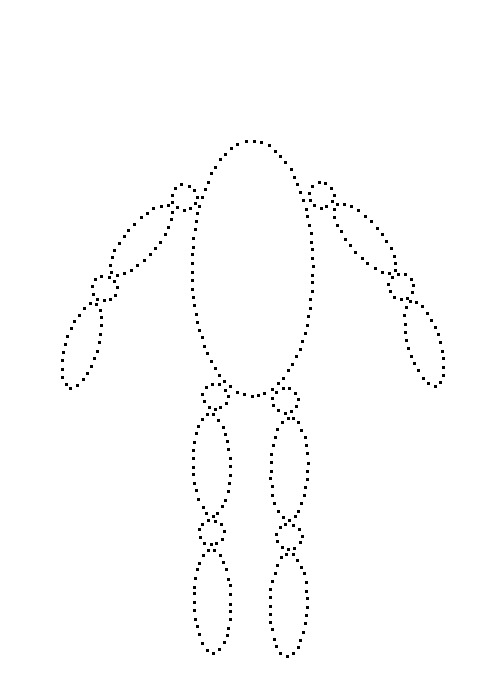
\includegraphics[width=0.40\textwidth]{InputPose1}} &	
		\fbox{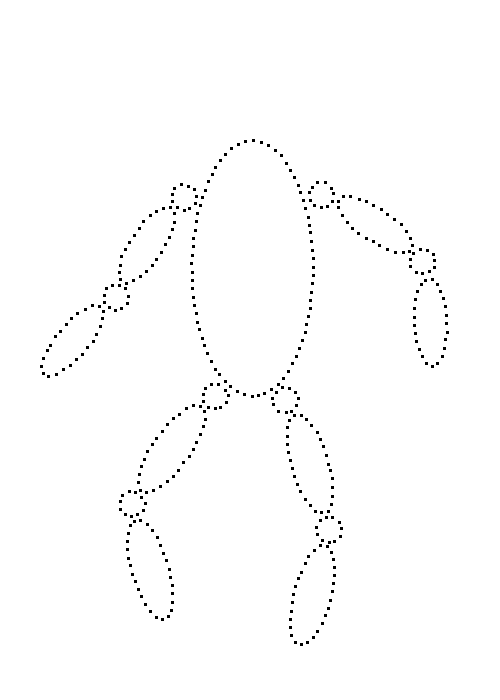
\includegraphics[width=0.40\textwidth]{InputPose2}} 
		\\
		(a) & (b) 
	\end{tabular}
	\caption{Taking an articulated object (puppet) in two different poses $C_1$ (a) and $C_2$ (b) in form of a 2D point cloud representing its hull point cloud as input.} 
	\label{fig:inputPoses}
\end{figure}
%%
\subsection{Implementation steps}
In order to re-implement the algorithm in 2D, only minor modifications concerning point coordinates and feature histograms had to be accomplished. The most crucial part of the whole algorithm is the initial alignment of $C_1$ and $C_2$ in order to detect the actual largest rigid part of the articulated object. This step is of particular importance, as the subsequent detection of further rigid parts proceeds from there. Therefore, as first step, sparse correspondences between $C_1$ and $C_2$ have to be detected (see subsection \ref{correspondences}). Furthermore, the detection of linked rigid parts to detected LRPs
\begin{enumerate}
	\item The PCA is employed on the input clusters $C_1$ and $C_2$ to estimate the normals of all points.
	\item Point feature histograms (FPFH) are computed to detect sparse point correspondences between $C_1$ and $C_2$. A Point correspondence between $C_1$ and $C_2$ needs to be \textit{reciprocal}.
	\item The RANSAC approach is applied on those correspondences to detect a $T_j$ that rejects wrong point correspondences. Clusters are detected from all corresponding points by applying region growing.
	\item The LRP is assigned to the resulting biggest point cluster.
	\item Proceeding with the LRP, unmatched clusters to $C_1$ and $C_2$ are seeked by region growing from the LRP. 
	\item Joints are estimated between the current LRP an all detected clusters from all unclustered points. Those are considered for allocating corresponding rigid parts of $C_1$ and $C_2$.
	\item Linked rigid parts are detected by rotating a cluster around its joint, given certain constraints and a calculating a weighted error.
\end{enumerate}

\subsection{Detection of sparse correspondences}
\label{correspondences}

As a first step of the algorithm, the normal as well as the feature histogram for each point of $C_1$ and $C_2$ (see section \ref{FPFH}) is computed. Results of the normal flipping procedure can be seen on figure \ref{fig:normalFlipping}.

%TODO: Picture of normal estimation + flipping
\begin{figure}[H]
	\centering\small
	\begin{tabular}{cccc}
		\fbox{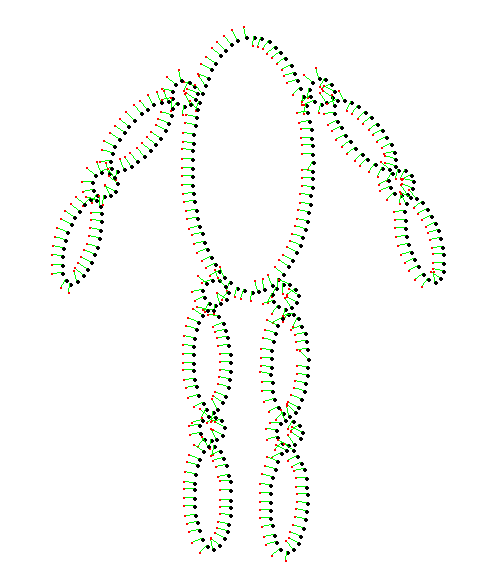
\includegraphics[width=0.23\textwidth]{Normals_C1_cropped}} &	
		\fbox{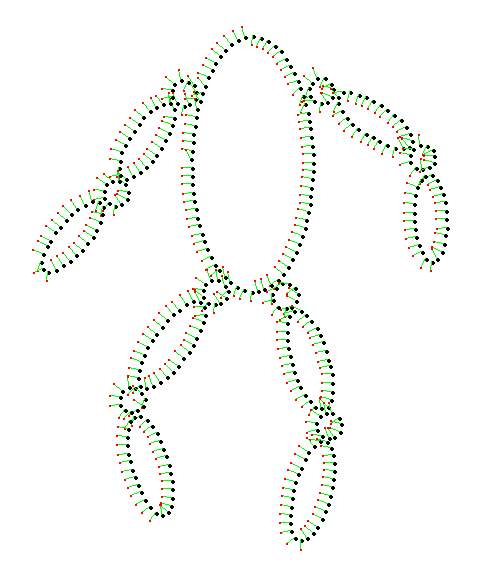
\includegraphics[width=0.23\textwidth]{Normals_C2_cropped}} &	
		\fbox{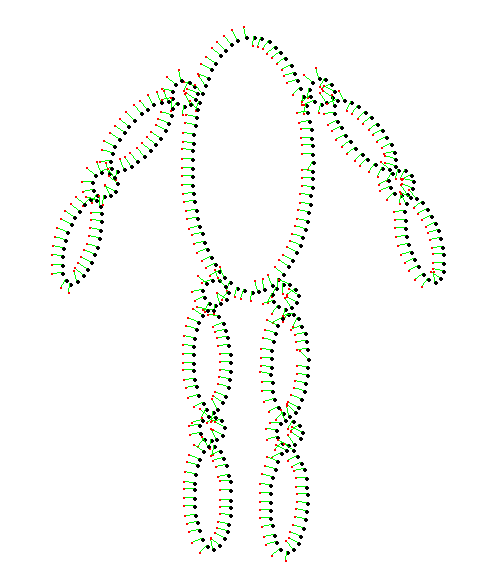
\includegraphics[width=0.23\textwidth]{Normals_C1_cropped}} &	
		\fbox{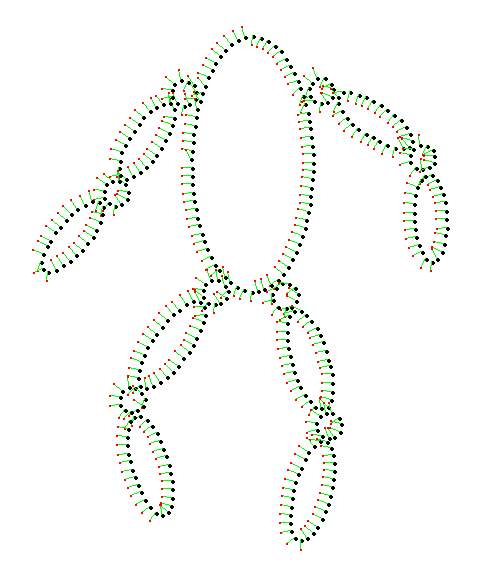
\includegraphics[width=0.23\textwidth]{Normals_C2_cropped}} 
		\\
		(a) & (b) & (c) & (d)
	\end{tabular}
	\caption{Normal estimation of two Cluster $C_1$ and $C_2$ (a) and (b) a subsequent global traversing of all normals to orient them similar (c) and (d).} 
	\label{fig:normalFlipping}
\end{figure}

It can be observed that the flipping of normals does not successfully globally flip all normals. The reason are narrow positions where the edges of two rigid parts almost touch and form a corner, like the armpits. In this case the normals get flipped although they should not. For this reason the global flipping of the normals lead to more false point correspondences.

For the detection of sparse correspondences between $C_1$ and $C_2$ three histogram distances (see section \ref{histogramCriteria}) are taken into account. Two point are selected as correspondences if their feature histogram they are \textit{reciprocal}. Depending on the chosen distance as criteria, more or less correspondences can be detected, refer to section \ref{ResultsLRP} for a detailed comparison. The mean histogram of all histograms as well as a \textit{unique} histogram can be seen on \ref{fig:meanHistogram}. 
%%
%TODO: Picture of mean histogram + similar histogram
%%
\begin{figure}[H]
	\centering\small
	\begin{tabular}{cc}
		\fbox{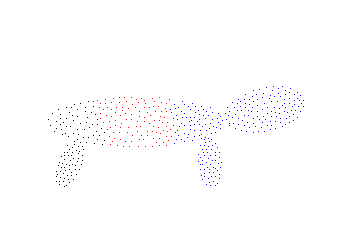
\includegraphics[width=0.45\textwidth]{results/4_1parts_clusters_rigidParts_7th}} &	
		\fbox{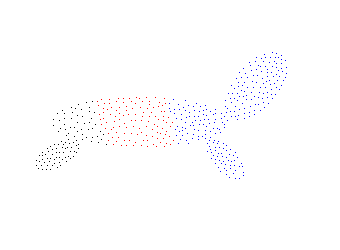
\includegraphics[width=0.45\textwidth]{results/4_2parts_clusters_rigidParts_7th}} 
		\\
		(a) & (b) 
	\end{tabular}
	\caption{Computing of the $\mu$ histogram of $C_1$ (a) in order to reject frequently emerging feature histograms (b) being inside a value $\mu \pm \theta \cdot \sigma$.} 
	\label{fig:meanHistogram}
\end{figure}
Figure \ref{fig:sparseCorrespondences} represents the resulting point correspondences from feature matching. It is clearly evident that points being located in a corner are more likely to detect a reciprocal point correspondence than points located at smooth surfaces. The reason is, that those features appear considerable similar which makes it difficult to distinguish them.
%%
\begin{figure}[H]
	\centering \small
	\begin{tabular}{c}
		\fbox{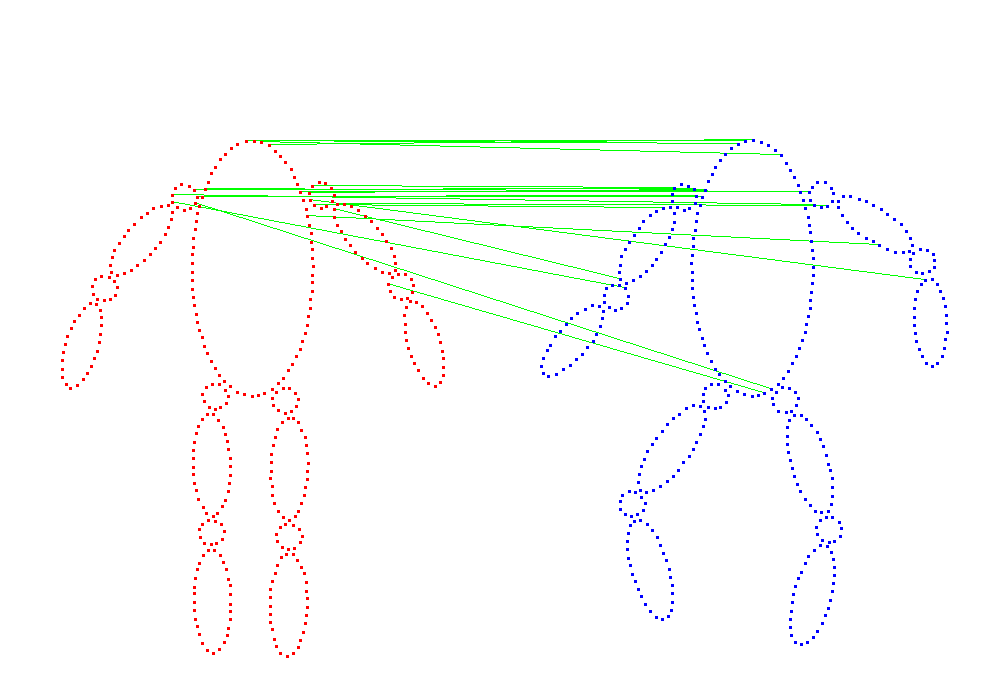
\includegraphics[width=0.80\textwidth]{featureCorrespondences_chiSquare}} 
	\end{tabular}
	\caption{Visualization of the point correspondences established from most similar, reciprocal feature histograms using the chi-square distance between all points of $C_1$ (red) and $C_2$ (blue).}
	\label{fig:sparseCorrespondences}
\end{figure}
%%
As some of those correspondences might be wrong, a RANSAC approach is applied on all correspondences to reject false ones (see subsection \ref{detectionLRP}).
%%
\subsection{Detection of the largest rigid part}
\label{detectionLRP}
The dense point correspondences from the previous computation step (see subsection \ref{correspondences}) may contain several errors. Therefore, RANSAC is applied as a next step to detect a single rigid transformation $T$ that leads to the biggest overlapping point cluster of $C_i$ and $C_j$. Thereby, in each iteration, 2 random correspondences are selected and used for the calculation of $T$ which is applied on $C_i$ to be translated on $C_j$. The number of iterations highly depends on the ratio of right and wrong point correspondences. Based on visual assessments, the number of iterations was set to 500.
%%
%TODO: number of iterations? --> number of false correspondences, formular
%%
Subsequently, clusters are grown from all corresponding points with an euclidean distance $d(\boldsymbol{p}_i,\boldsymbol{p}_j)$ again below a predefined threshold $\tau$. The procedure is applied both on $C_i$ and $C_j$ which results in two rigid parts as output (see figure \ref{RANSAC}).

\begin{figure}[H]
	\centering\small
	\begin{tabular}{cc}
		\fbox{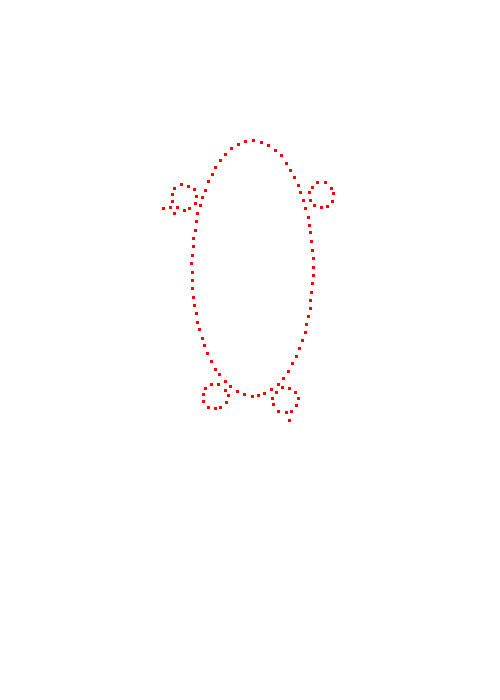
\includegraphics[width=0.40\textwidth]{RANSAC_1000_chiSquare_ref}} &	
		\fbox{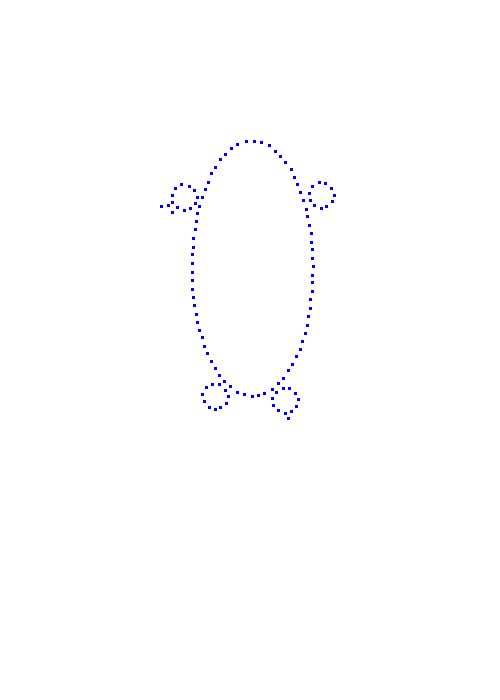
\includegraphics[width=0.40\textwidth]{RANSAC_1000_chiSquare_target}} 
		\\
		(a) & (b) 
	\end{tabular}
	\caption{Computation of the largest rigid part from $C_1$ (a) and $C_2$ (b) by applying RANSAC on the detected point correspondences.} 
	\label{fig:RANSAC}
\end{figure}

The final transformation $T$ of the RANSAC approach, which leads to the ``largest rigid part'', is applied on the reference cluster. This procedure is required in order to similarly align $C_1$ and $C_2$ for further computations (see subsection \ref{CorrespondingClusters}).

\subsection{Cluster detection by region growing}
\label{cluster}
After successfully detecting a ``largest rigid part'' $P_i$ and $P_j$ for each input clusters $C_i$ and $C_j$ they are added to a list of rigid parts $\mathcal{P}$. Potential linked rigid parts are detected from region growing of all unclustered points $\mathcal{U} =  \{\boldsymbol{u}_1,\ldots,\boldsymbol{u}_n\}$. Those comprise all cluster points of $C_1$ and $C_2$ excluding already detected largest rigid parts $\mathcal{P}$. The region growing initiates with the first point $\boldsymbol{u}_1$ of the unclustered points $\mathcal{U}$ to form a cluster $C_i$. Another point of the unclustered points $\boldsymbol{u}_j$ is added to $C_i$, if the euclidean distance $d(\boldsymbol{p}_i,\boldsymbol{u}_j)$ to any point in $C_i$ is below the threshold $\tau$. If no further unclustered points can be added, the region growing initiates again with the first unclustered point $\boldsymbol{u}_1$ that has not been added by region growing until all points traversed the procedure. The result is a set of clusters $\mathcal{C}$ for each $C_i$ and $C_j$. Subsequently, a preliminary joint $\boldsymbol{j}_i$ for each output clusters is stored, by detecting the two nearest points of $C_i$ and $P_i$. The joints are required for following cluster correspondence and joint weights for the ICP (see subsection \ref{CorrespondingClusters} and \ref{JointWeights}).

\subsubsection{Establishment of corresponding clusters}
\label{CorrespondingClusters}
In case of detecting more than one cluster for each $C_i$ and $C_j$, which might be for example the case for the extremities linked to the torso, it must be verified which clusters correspond to each other. This step is essential, as the algorithm is called recursively (starting from \ref{correspondences}) with two new input clusters. Thereby, the provisional joints $\boldsymbol{j}_i$ are used to associate two clusters of $C_i$ and $C_j$ by detecting the closest joint with the euclidean distance $d(\boldsymbol{j}_i,\boldsymbol{j}_j)$.

\subsection{Detection of linked rigid parts}
\label{JointWeights}
In the reference paper the feature matching in combination with RANSAC for detecting correspondences was reapplied on the linked clusters to the already detected rigid parts. However, this approach is not successful in the current 2D application. The reason is that the point features are not meaningful due to the reduced number of points and the shapes are too similar. In order to iteratively detect further rigid parts linked to already detected ones another approach was developed which manages to avoid another time-consuming RANSAC. Thereby, the knowledge is used that the rigid parts are transformed by rotating around a joint. For that purpose the estimated joints $\mathcal{J} = j_1,\cdots,j_n$ resulting from \ref{cluster} are taken into account. As a first step, two input clusters $C_i$ and $C_j$ are transformed that their joints overlap. Next, the primary axis of $C_i$ and $C_j$ are aligned to guess an initial alignment which should further reduce the computation steps. Then, $C_i$ is iteratively rotated around its joint into the direction of an decreasing least squares error $e$ (to overlap with $C_j$). By iteratively updating $e$ after each rotation step, a best overlapping position between the linked rigid parts can be detected. Thereby, the preliminary joints are used as weights. As a consequence, a point $p_i$ being located far away from its allocated joint $J_n$ does not contribute as much to the matching error as points located near the joint. A weight $w$ is calculated by comparing the distance $d(p_i, J_n)$ to the maximal distance $d_{max}$ between $J_n$ and the farthermost allocated point. Subsequently a total matching error $e$
%
\begin{equation}
\begin{split}
w_i = \| \boldsymbol{p}_i - \boldsymbol{j}_n\| \cdot \frac{1}{d_{max}}
\\
e = \displaystyle\sum_{i=1}^{m}\| \boldsymbol{p}_i - \boldsymbol{q}_i\|^2 \cdot (1 - {w_i})^2
\end{split}
\label{eq:jointWeightError}
\end{equation}
%
is achieved by combining the distance of a point to its closest point and the joint weight $w$. The error is squared in order to further weaken the influence of cluster points being located far away from the joint. The final correspondence equals to the biggest cluster resulting from rotation around the joint $\boldsymbol{j}_i$ with a minimum error $e$. As a last step, all points with a closest point below a certain threshold $\tau$ are taken as input for region growing. It is assumed, that two linked rigid parts are quite similar aligned, therefore the distance threshold $\tau$ is considerable small. The largest cluster is finally returned as detected linked part.
%%
\begin{figure}[H]
	\centering\small
	\begin{tabular}{ccc}
		\fbox{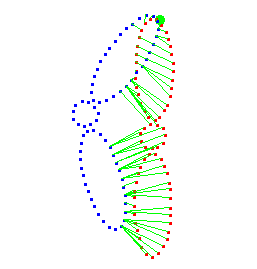
\includegraphics[width=0.30\textwidth]{LegRotation_Before_cropped}} &	
		\fbox{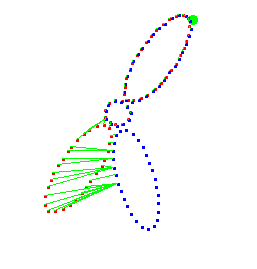
\includegraphics[width=0.30\textwidth]{LegRotation_After_cropped}}  &	
		\fbox{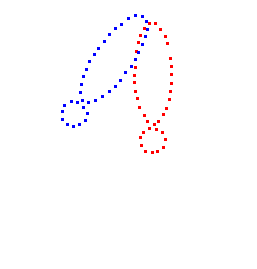
\includegraphics[width=0.30\textwidth]{LegRotation_Results_cropped}} 
		\\
		(a) & (b) & (c)
	\end{tabular}
	\caption{The joints $J_i$ and $J_j$ (green dots) of the reference cluster $C_i$ (red) and the target cluster $C_j$ (blue) are overlapped. The closest points for $C_i$ are computed (a). Stepwise rotation of $C_i$ onto $C_j$ in the direction of a decreasing error until $e$ does not further decrease (b). Final overlapping clusters from taking all closest points of $C_i$ and $C_j$ below a distance threshold $\tau$ (c).} 
	\label{fig:jointRotation}
\end{figure}
%%
With varying distance thresholds $\tau$ for achieving the final cluster, points from the actual target are skipped or unnecessary points from another rigid part are added. Those circumstances lead to difficulties for the detection of linked parts. Detailed results about this appearance can be seen in section \ref{ResultsLRP}.

\section{Implementation}
\label{ImplementationLRP}
For the implementation in Java the individual steps of the largest rigid part algorithm have been split into individual classes for a better overview. Again ImageJ was used as processing library, which only gets a stack with two point clouds as input.
%
%TODO: Add class graph of implementation
%
The whole algorithm initiates from the \texttt{Segmentation} class, where all steps proposed in \ref{LRP} are implemented. Basically, the segmentation proceeds until no unclustered points can be detected or no clusters need to be processed. In the beginnin of the loop already detected rigid parts are removed from the unclustered points (\texttt{removeAllLRPs()}). As a next step clusters are detected either for the initial point cloud or in case of linked parts for an LRP. Joints are only estimated for the clusters in case of a detected rigid part which is the case for all iterations except the first one. Then, all clusters are added to the \texttt{Stack} by detecting matching ones (\texttt{pushMatchingClusters()}). In case of an empty stack, all clusters have been processed and the algorithm terminates. On the other hand, two matching clusters are popped from the Stack and are segmented with the next steps.

\begin{lstlisting}
while (unclusteredReference.size() > MIN_SIZE || !clusters.isEmpty()) {

	removeAllLRPs();

	referenceClusters = RegionGrowing.detectClusters(unclusteredReference);
	targetClusters = RegionGrowing.detectClusters(unclusteredTarget);

	if (currentLrps != null) {
		detectJoints(currentLrps, referenceClusters, targetClusters);
	}

	if (referenceClusters.size() != 0 && targetClusters.size() != 0) {
		pushMatchingClusters();
	}

	if (clusters.isEmpty()) {
		return;
	}

	currentClusters = clusters.pop();

	if (currentClusters[0].getJoint() == null) {
		FeatureMatching fm = new FeatureMatching(currentClusters[0], currentClusters[1]);
		Map<Integer, Integer> denseCorrespondances = fm.getCorrespondences();

		if (denseCorrespondances.size() < 3) {
		return;
		}

		RANSAC ransac = new RANSAC(currentClusters[0], currentClusters[1], denseCorrespondances);
		currentLrps = ransac.getLargestRigidParts();
		unclusteredReference = ransac.getTransformedReferencePoints();
	}

	else {
		PartDetection pd = new PartDetection(currentClusters[0], currentClusters[1]);
		currentLrps = pd.getLinkedParts();
	}

	if (currentLrps[0].getPoints().size() < 5) {
	} else {
	largestRigidParts.add(currentLrps);
	}
}
\end{lstlisting}

\subsection{Feature Detection}
As a first step, the normals of all points $n$ of $C_1$ and $C_2$ are computed. For this matter the class \texttt{NormalEstimation} was developed that takes a point $p_i$ with its $k$ neighbors as input. In my case only 2 neighbors are selected. Then, the least fitting error line on those input points is detected (as described in section \ref{correspondences}) and the smallest lambda value $\lambda_2$ selected as eigenvalue. By setting the x-value of the normal to 1.0, the y-value can be calculated with the eigenvalue $\lambda_2$. The resulting vector represents the normal vector $\vec{n}$ for $p_i$. In case of being exactly vertically or horizontally, the resulting value for y is either infinite or not a value (Nan), in these cases the normal is set to (0,1) or (1,0). As a last step, the normal is normalized.
%%
\begin{lstlisting}
double eigenvalue = Math.min(lambda1, lambda2);

	covarianceMatrix = new double[][] { 
		{ a - eigenvalue, b},
		{ b, c - eigenvalue}
	};

double[] normal = new double[2];

normal[0] = 1.0;
normal[1] = (eigenvalue * normal[0] - covarianceMatrix[0][0] * normal[0])/covarianceMatrix[0][1];

if(Double.isInfinite(normal[1])){
	normal[0] = 0;
	normal[1] = 1;
} else if (Double.isNaN(normal[1])){
normal[1] = 0;
}

double length = Math.sqrt(Math.pow(normal[0], 2) + Math.pow(normal[1], 2));
		
normal[0] /= length;
normal[1] /= length;
point.setNormal(normal);
\end{lstlisting}
%%
A \texttt{ClusterPoint} was implemented to store the normal $n_i$ for each point and the resulting feature histogram (FPFH) in form of a \texttt{Histogram} object containing a \texttt{int[]} array. For the calculation of a feature histogram of a point $p_i$, its $k$ neighbors are taken into account. The \texttt{FPFH} class implements various operations for vectors, like a dot or cross product to implement the formula from subsection \ref{FPFH}.
%%
\begin{lstlisting}
public void featureHistogram(p_i) {
	SPFH = SPFH(p_i);

	for (ClusterPoint p_k : p_i.getNeighborhood()) {
		double weight = p_i.distance(p_k);
		weightedSPFH = weightedSPFH.addHistograms(SPFH(p_k).multiplyHistograms(1.0 / weight));
	}
	
	FPFH = SPFH.addHistograms(weightedSPFH.multiplyHistograms(1.0 / p_i.getNeighborhood().size()));
	
	p_i.setFPFH(FPFH);
}
\end{lstlisting}
%%
For the comparison of two feature histograms from $C_1$ and $C_2$ only unique ones are considered. Point correspondences are calculated by detecting a corresponding point from $C_2$ for an input point $p_i$ of $C_1$ applying a distance on the feature histograms (see section \ref{correspondences}). The distance can be chosen by the user.
%%
\begin{lstlisting}
private int closestPoint(ClusterPoint p_i, List<ClusterPoint> c_2) {
	int closestPoint = -1;
	double distance = Double.MAX_VALUE;
	double distanceNew = 0;
	
	for (int i = 0; i < c_2.size(); i++) {
	
		if (Input.distance.equals("Euclidean")) {
			distanceNew = p_i.getFPFH().squaredDistance(c_2.get(i).getFPFH());
		} else if (Input.distance.equals("ChiSquared")) {
			distanceNew = p_i.getFPFH().chiSquare(c_2.get(i).getFPFH());
		} else {
			distanceNew = p_i.getFPFH().kullback(c_2.get(i).getFPFH());
		}
	
		if (distanceNew < distance) {
		distance = distanceNew;
		closestPoint = i;
		}
	}
	return closestPoint;
}
\end{lstlisting}
%%
Reciprocal point correspondences between $C_1$ and $C_2$ are returned in form of point indices \texttt{Map<Integer,Integer>}  of the clusters cluster points.
%%
\begin{lstlisting}
for (Map.Entry<Integer, Integer> entry : reference.entrySet()) {
	Integer referenceIndex = entry.getKey();
	Integer targetIndex = entry.getValue();

	ClusterPoint currentRefPoint = originalReference.get(referenceIndex);
	ClusterPoint currentTargetPoint = originalTarget.get(targetIndex);
...
	if ((reciprocalMatching && target.get(targetIndex) == referenceIndex){

		finalReferencePoints.add(currentRefPoint);
		finalTargetPoints.add(currentTargetPoint);
		finalAssociations.put(referenceIndex, targetIndex);
	}
}
\end{lstlisting}
%%
%TODO: add algorithm of FPFH + normals
%%
\begin{algorithm}[tbp]
	\caption{Computation of the normal and subsequently feature histograms of a cluster point $p_i$ with its $k$ neighbors inside a radius $r$. The fast point feature histograms FPFH are computed by weighting the SPFH of a $p_i$ and its $k$ neighbors.}
	
	\begin{algorithmic}[1]     % [1] = all lines are numbered
		\label{featureHistograms}
		
		\Procedure{FPFH}{$p_i$} 
		\State $\mathit{C_{max}} \gets ()$
		\State $\mathit{C_{current}} \gets ()$
		\State $n \gets \mathit{sizeOf}(M)$
		\State $m \gets \mathit{sizeOf}(C_{current})$
		
		\While {$n$ > 0}
		\State $\mathit{c_{current}} \gets \mathit{c_{current}} + \boldsymbol{u}_1$
		\For{$i = 1,\ldots,m$}
		\State $M \gets M - C_{current}$
		\For{$j = 1,\ldots,n$}
		\If {\Call{$d$}{$\boldsymbol{p}_i, \boldsymbol{u}_j}< \tau$}
		\State $C_{current} \gets C_{current} + \boldsymbol{u}_j$
		\EndIf
		\EndFor
		\EndFor
		\State $M \gets M - C_{current}$
		\If{$m > \mathit{sizeOf}(C_{max})$}
		\State $C_{max} \gets C_{current}$
		\EndIf
		\State $C_{current} \gets ()$
		\EndWhile
		\State\Return $C_{max}$
		\EndProcedure	
	\end{algorithmic}
\end{algorithm}
%%
%TODO: add code snippet of feature calculation

\subsection{RANSAC}
\label{RANSAC}
The RANSAC algorithm takes the computed dense correspondences between $C_i$ and $C_j$ in form of a \texttt{Map<Integer, Integer>} as input. As a first step, three random correspondences are selected from the map to calculate an affine transformation between the three resulting points from each $C_i$ and $C_j$. The initial orientation and alignment is thereby irrelevant as the transformation $T$ is completely recalculated.
%%
\begin{lstlisting}
public LargestRigidPart(Cluster c_i, Cluster c_j, Map<Integer, Integer> correspondences)
...
points1 = c_i.getPoints();
points2 = c_j.getPoints();
...
private void getRandomPoints(int num) {
	Integer[] keys = correspondances.keySet().toArray(new Integer[0]);
	Integer[] values = correspondances.values().toArray(new Integer[0]);

	for (int i = 0; i < num; i++) {
		index = (int) (Math.random() * correspondances.size());
		randomPoints1.add(points1.get(keys[index]));
		randomPoints2.add(points2.get(values[index]));
	}
}
...
\end{lstlisting}
%%
In each iteration on all point correspondences a region growing approach with a threshold $\tau$ is conducted. The value is thereby considerably small as a right alignment during any iteration is assumed. The biggest cluster is stored and after all iterations returned as largest rigid part. The whole RANSAC procedure is quite time consuming. It can be reduced by taking a smaller number of correspondences as input which directly affects the required number of iterations until a right match is detected (see \ref{ResultsLRP}).

\subsection{Region growing}
\label{RegionGrowing}
The region growing algorithm is quite similar to the earlier described algorithm (see algorithm \ref{noiseRemoval}). There is also an adaptation, which does not only return the largest cluster, but all clusters above a certain size. The detected clusters are handled in a \texttt{Stack<Cluster>} in case of more than one detected clusters. Thereby, all clusters are pushed on the stack. With each recursion two corresponding cluster $C_i$ and $C_j$ are popped from the stack and taken as input for the whole algorithm. If again more clusters are detected they are pushed on the stack and treated before recently added clusters.

\subsection{Joint rotation}
The main part for the detection of linked parts to already detected rigid parts is the rotation of $C_i$ onto $C_j$. As a first step both clusters are moved to the origin and are similarly aligned.
%%
\begin{lstlisting}
if (c_i.getJoint() != null) {
	referencePoints = Matrix.translate(c_i.getPoints(), -c_i.getJoint().getX(), -c_i.getJoint().getY());
	targetPoints = Matrix.translate(c_j.getPoints(), -c_j.getJoint().getX(), -c_j.getJoint().getY());
	initialOrientation(c_i.getJoint());
	}
\end{lstlisting}
%%
As a next step, the reference points are aimed to be rotated onto the target points. This is achieved iteratively by applying a rotation in the direction of an achieved reduced error. By computing an error for each iteration, the assumed biggest overlap is achieved.
%%
\begin{lstlisting}
for (Map.Entry<Integer, Integer> entry : correspondences.entrySet()) {
...
	totalError += currentError / referencePoint.distance(new ClusterPoint(0,0));	
...	
}
\end{lstlisting}
%%
To only remain the rigid part and reject correspondences from the final corresponding points that do not belong to the searched part, a region growing algorithm is applied to only keep the largest cluster as successful detected rigid part (see subsection \ref{RegionGrowing}).

\section{Results}
\label{ResultsLRP}

Applying the proposed approach on the 2D data set of an articulated object, following results could be achieved. Alternative results (reducing k neighbors, histogram bins, histogram criteria) could be achieved --> Compare runtime of criteria + number of right correspondences as percentage.

%TODO: add pictures of LRP results

\subsection{Histogram similarity criteria}
The chosen distance between histograms is essential. Euclidean --> most correspondences, more iteration in RANSAC but certainly right more right ones.
Chi-Square --> less correspondences, more right ones, less iterations with RANSAC
Kullback-Leibler --> few correspondences, LRP might not be detected as too few right ones
Not useful in this context, more points required
%TODO: runtime + pictures!

\subsection{Main difficulties}
The main drawback of the algorithm represents the first initial alignment of the two poses of the articulated object. In case of a failure, the linked parts can not be detected right as they are computed from region growing. By increasing the number of RANSAC iterations, the probability of a faulty initial alignment can be reduced, however this directly affects the runtime and should therefore not be exaggerated. Most certainly, it has to be guaranteed that the number of corresponding points are the same number from $C_1$ and $C_2$.

%TODO: picture faulty alignment

As the input point cloud of an articulated object is in 2D, the imitation of the object's hull is required. As a consequence, the region growing is much more error-prone, as unlikely in 3D, the points of a rigid part have a considerable lower number of neighbors. In case of a few missing cluster points from a rigid part, it will not be fully detected during the region growing due to the gaps which is especially drastically during the RANSAC approach. To counteract this behavior, more and closer hull points could added to each rigid part, that more links for region growing are available. A further main problem is that the algorithm proceeds iteratively from already detected rigid parts. This makes the whole procedure quite unstable and error prone, as one faulty detection leads to an overall unsuccessful segmentation of an articulated object. In the implementation of Mitra enough feature descriptors were available for linked rigid parts, that they could be detected similary as the initial alignment. But for that more data points have to be available which is not the case for this prototype.

Furthermore, touching of rigid parts (e.g. the hand touches the leg) constitute difficulties as the region growing would not detect those as potential linked clusters.

%TODO: show what does not work perfectly

\section{3D implementation}

The next step would be to implement the approach in 3D. A similar implementation was done by Mitra \cite{Mitra07} (see section \ref{functionalityLRP}) by using the PCL. Most essential functions like FPFH and subsampling for large point clusters are already provided. A good dataset would be thereby the SCAPE, which offers different poses of a scanned human. 

%TODO: Write what fails/main problems/solutions







